\documentclass{article}
\usepackage{graphicx}
\usepackage{xcolor}
\usepackage{ bbold }
\usepackage[margin=0.8in, a4paper]{geometry}
\usepackage{amsmath} 
\usepackage{amssymb}
\title{Rotation-symmetric bosonic codes}
\author{Tien Nguyen Dinh}
\date{February 2024}
\graphicspath{{images/}}
\DeclareMathOperator{\lgcZ}{\bar{Z}}
\DeclareMathOperator{\lgcX}{\bar{X}}
\DeclareMathOperator{\lgczero}{|\bar{0}\rangle}
\DeclareMathOperator{\lgcone}{|\bar{1}\rangle}
\DeclareMathOperator{\lgcplus}{|\bar{+}\rangle}
\DeclareMathOperator{\lgcminus}{|\bar{-}\rangle}
\DeclareMathOperator{\lgcpm}{|\bar{\pm}\rangle}
\DeclareMathOperator{\tr}{\text{tr}}
\DeclareMathOperator{\diag}{\text{diag}}
\DeclareMathOperator{\CR}{\text{CR}}
\DeclareMathOperator{\psianc}{|\Psi_{\text{anc}}\rangle}
\DeclareMathOperator{\psidata}{|\Psi_{\text{data}}\rangle}


\begin{document}

\maketitle

\section{Introduction}
Bosonic codes are a broad class of bosonic error-correcting codes based on phase-space rotation symmetry [We'll soon know that Fock spacing is the \textit{necessary} condition for phase-space rotation symmetry]. The idea is simple: quantum information can be encoded into bosonic systems instead of discrete two-level systems. The infinite Hilbert space of a single bosonic mode provides the playground for redundancy.

From a hardware perspective, such a bosonic system can be realized in optical cavities \cite{kimble1998_cavityQED}, where bosonic modes are the modes of the electromagnetic field, superconducting microwave cavities \cite{gao22_squeezed}, or ion traps. 

The RSBC are different from the GKP code \cite{gkp01} in the sense that, while RSBC makes use of rotational phase-space symmetry for noise protection, GKP codes make use of discrete translation. Experimentally speaking, RSBC codes, most notably cat and binomial code, are progressing much faster than the GKP code. 

Formally speaking, RSBC codes are bosonic codes characterized by discrete rotation symmetry in phase space. A single qubit is encoded into a subspace in which the discrete rotation operator $\hat{Z}_N=\exp[i(\pi/N)\hat{n}]$ acts as a logical $\bar{Z}$. The parameter $N$ denotes the degree of discrete rotation symmetry. It follows that the identity is straightforwardly $\hat{R}_N=\bar{Z}^2$ [from a stabilizer formalism perspective, $\hat{R}_N$ is the code's stabilizer]. A direct consequence of $N$-fold rotation symmetry is that the logical state $|\bar{\psi}\rangle$ has support only on every $N$-th Fock state, $|\bar{\psi}\rangle=\sum_{k=0}^\infty c_{kN}|kN\rangle$. The degree of rotation symmetry $N$ thus quantifies the magnitude of a detectable shift in number and naturally sets a code distance [between the two logical states] in Fock space. A complimentary notation of distance in phase space is $\pi/N$, which quantifies detectable number-shift and rotation errors [if you think about it, an error that causes a $Z$ rotation of $\pi/N$ will not be detectable, because you're still in the codespace]. 

\section{Bosonic rotation codes}
A code has discrete $N$-fold rotation symmetry if any state $|\bar{\psi}\rangle$ is a $+1$ eigenstate of the discrete rotation operator 
\begin{align}
    \hat{R}_N = e^{i(2\pi/N)\hat{n}},
\end{align}
where $\hat{n}=\hat{a}^\dagger \hat{a}$ is the Fock-space number operator. An order-$N$ bosonic rotation code is a code where the operator 
\begin{align}
    \hat{R}_{2N} = e^{i(\pi/N)\hat{n}} 
\end{align}
acts as a logical $\bar{Z}$ gate. The logical codewords are therefore clear. They can be constructed from discrete rotated superpositions of a normalized \textit{primitive} state $|\Theta\rangle$. Since $\lgcZ\lgczero=\lgczero$ and $\lgcZ\lgcone=-\lgcone$, the logical codewords must be 
\begin{align}
    \lgczero = \dfrac{1}{\sqrt{\mathcal{N}_0}}\sum_{m=0}^{2N-1}e^{i(m\pi/N)\hat{n}}|\Theta\rangle,\\
    \lgcone = \dfrac{1}{\sqrt{\mathcal{N}_1}}\sum_{m=0}^{2N-1}(-1)^m e^{i(m\pi/N)\hat{n}}|\Theta\rangle,
\end{align}
where $\mathcal{N}_i$ are the normalization constants. There's some constraints on how the primitives are defined, but we'll look at them later. For now, let us take them as valid states, then the codewords themselves are exactly orthogonal and the normalization constants are different. It follows that a superposition of the logical states are $N$-fold symmetric too. 
As an example, the cat code, which is a RSBC code, is constructed from a coherent state $|\Theta\rangle = |\alpha\rangle$ [\textit{A coherent state}, mathematically, is the eigenstate of the annihilation operator $\hat{a}$; physically, a coherent state remains unchanged by the annihilation of field excitation; moreover, when expressed in the energy basis ($|n\rangle$) it follows a Poisson distribution]. 
\subsection{Fock-space structure}
As mentioned, discrete rotation symmetry enforces Fock spacing: the fact that a logical state $|\bar{\psi}\rangle$ of order-$N$ code has support only on $N$-th states in the Fock space. 
This link can logically derived as follow. Let us have an arbitrary state $|\psi\rangle = \sum_n a_n|n\rangle$. If such a state is a $+1$ eigenstate of the logical $Z$ operator, then
\begin{align}
    e^{i(\pi/N)\hat{n}} \sum_n a_n |n\rangle = \sum_n e^{i(\pi/N)n}a_n|n\rangle = \sum_n a_n |n\rangle
\end{align}
For this to be true, $a_n=0$ for every $n\neq 2kN$. For every $n=2kN$, the amount of rotation is $\pi/N\times 2kN=2k\pi$, which is essentially identity for integer $k$. A similar argument can be said for the $-1$ eigenstate of the logical $Z$ operator. In short, the logical codewords written in the photon number Fock basis is 
\begin{align}
    \lgczero = \sum_{k=0}^{\infty} f_{2kN}|2kN\rangle,\\
    \lgcone = \sum_{k=0}^{\infty} f_{(2k+1)N}|(2k+1)N\rangle. 
\end{align}
Now, the coefficients $f_{kN}$ are related to the Fock-state coefficients of the primitive $|\Theta\rangle=\sum_n c_n|n\rangle$. The exact connection can be found in the RSBC code paper.
To bridge between the two phase-space and Fock-space pictures, we make use of the Kronecker comb, 
\begin{align}
    \dfrac{1}{M}\sum_{m=0}^{M-1}e^{2\pi m n/M} = \sum_{k=0}^{\infty}\delta_{n, kM},
\end{align}
First, let us construct a rank-2 projector onto the set of Fock states $|2kN+\ell\rangle$, $k$ integer. $\ell = 0$ or $N$, representing the supporting number states of the logical zero and one respectively.
\begin{align}
    \hat{\Pi}^\ell_{2N} &= \sum_{k=0}^\infty |2kN+\ell\rangle \langle 2kN+\ell|\\
    &=\dfrac{1}{2N}\sum_{m=0}^{2N-1}(e^{-i(\pi\ell/N)}\hat{Z}_N)^m
\end{align}
Then,
\begin{align}
    \lgczero_{Fock} \propto \hat{\Pi}^0_{2N}|\Theta\rangle,\\
    \lgcone_{Fock} \propto \hat{\Pi^N_{2N}}|\Theta\rangle. 
\end{align}
The dual-basis codewords $\lgcpm$ are constructed as usual, $\lgcpm=(\lgczero\pm \lgcone)/\sqrt{2}$. Both of them have support on the full set of $|kN\rangle$ Fock states. 

A useful quantity for comparing codes is the average excitation number of the code,
\begin{align}
    \bar{n} = \dfrac{1}{2}\text{tr}[\hat{\Pi}\hat{n}]
\end{align}
where $\hat{\Pi}$ is a two-dimensional projector onto the codespace. By construction, the average excitation number is the same for each of the dual-basis codewords [That's for sure, because both have equal-in-magnitude Fock coefficients]. It should be noted that since the rotation operator commutes with the number operator, rotations do not change the excitation number. 
\subsection{The phase and Fock grids}
Given a primitive $|\Theta\rangle$, the order of rotation symmetry $N$ parameterizes a code both in phase space and in Fock space. From these two forms of the codewords, we have a number distance and rotational distance of a code as 
\begin{align}
    d_n = N,\quad d_\theta=\pi/N,
\end{align}
respectively. Since they are inversely proportional, a code of increasing number distance will be vulnerable to phase errors as they have at the same time a closely separation in phase space. For an order-$N$ rotation code, we refer to the set of angles $\{md_\theta\}$ for $m=0, 1,\dots, 2N-1$ as the phase grid and the set of Fock states $\{|kN\rangle\}$, $k=0,1,\dots$ as the Fock grid.  The position- and momentum-space grids of GKP codes carry the same interpretation.

The Fock grid and phase grid broadly characterize the types of error to which the code is naturally resilient. A number-shift error smaller than $d_n=N$ should be detectable, for an order-$N$ code. A phase error is more difficult to characterize, but in general a phase error $\delta$ which is small comparable to $d_\theta$ should also be detectable.
\subsection{Distinguishing the codewords}
\subsubsection{Number measurement}
The computational-basis codewords $\lgczero$ and $\lgcone$ can be distinguished by measuring the excitation number, $\langle \hat{n}\rangle$. It's obvious to see that, for an order-$N$ rotation code, a number measurement results in $kN$, where even integer $k$ corresponds to $\lgczero$ and conversely odd integer $k$ corresponds to $\lgcone$.
\subsubsection{Phase measurement}\label{phase_measurement}
Next, we need to think how to distinguish $\lgcpm$. The task is summarized as follows: Given the codeword $\lgcplus$ for a rotation code of order-$N$, we wish to determine $\theta$ in $e^{i\theta\hat{n}}|\lgcplus$. Then, once we know $\theta$, if $\theta$ mod $2\pi/N=0$, the state is $\lgcplus$, while if $\theta$ mod $2\pi/N=\pi/N$, the state is $\lgcminus$. In the presence of rotation errors, the phase estimation problem is generalized to estimating a continuous variable $\theta \in [0, 2\pi)$. A decoder rounds $\theta$ to the nearest $m\pi/N$. Then, if $m$ is even, declare the outcome plus, and vice versa. 

Holevo and Helstrom introduced an optimal \textit{measurement} to distinguish states in the one-parameter family $e^{i\theta\hat{n}}|\psi\rangle$ for the situation where no prior information about $\theta$ is assumed. The POVM of the measurement depends on a fiducial state $|\psi\rangle=\sum c_n|n\rangle$ that defines the phase-estimation problem, which in our case is the logical plus state. The POVM elements are
\begin{align}
    \hat{M}^{can}(\theta)=\dfrac{1}{2\pi}\sum_{m,n=0}^{\infty}\gamma_m\gamma_n^*e^{i(m-n)\theta}|m\rangle\langle n|.
\end{align}
For an order-$N$ rotation code, the relation $\hat{R}_N\lgcplus=e^{i2(\pi/N)\hat{n}}\lgcplus=\lgcplus$ implies that phase measurements only acquire information about the phase $\theta$ modulo $2\pi/N$ [Because $\hat{R}_N$ is the `stabilizer']. Because of this, the phase uncertainty of a measurement introduced by Holevo and Helstrom is also different. We can then define an uncertainty measure,
\begin{align}
    \Delta_N(\theta)=\dfrac{\langle\Delta e^{iN\theta}\rangle}{|\langle e^{iN\theta}\rangle|^2}=\dfrac{1}{|\langle e^{iN\theta}\rangle|^2}-1
\end{align}
where $\langle e^{iN\theta}\rangle$ is the mean modular phase. It can be calculated from the Fock-grid coefficients of the code,
\begin{align}
    \langle e^{iN\theta}\rangle = \int_0^{2\pi}e^{iN\theta}\mu(\theta)d\theta = \dfrac{1}{2}\sum_{k=0}^\infty |f_{kN}f_{(k+1)N}|
\end{align}
[I mean, strictly speaking, the expectation value of any quantity $M$ is calculated that way.] Experimentally speaking, phase measurements can be done by schemes like adaptive homodyne measurements or heterodyne measurement $|\alpha\rangle\langle\alpha|$. 
\section{Number-phase codes}
To minimize the uncertainty measure, we maximize the mean modular phase. It's straightforward to see that 
\begin{align}
    f_{kN}f_{(k+1)N} \leq \left(\dfrac{f_{kN}+f_{(k+1)N}}{2}\right)^2
\end{align}
and the mean modular phase $\langle e^{iN\theta}\rangle$ is maximized when the distribution of Fock-grid coefficients is completely flat, i.e when the `=' happens. From the normalization condition, it also implies that the maximum of the mean modular phase is unity, hence a vanished phase uncertainty. Such a state is however not physical. Formally we can consider familities of physical codes that in some appropriate limit satisfy $\Delta_N(\theta)\to 0$. 
\subsection{Ideal number-phase codes}
In analogy with ideal GKP codes defined in terms of superpositions of position (or momentum) eigenstates, we define a family of order-$N$ rotation codes as 
\begin{equation}\label{inp_codewords}
    \lgczero = \sum_{m=0}^{2N-1}|\phi=m\pi/N\rangle,\\
    \lgcone = \sum_{m=0}^{2N-1}(-1)^m|\phi=m\pi/N\rangle.
\end{equation}
where the fiducial states in this case are the phase states,
\begin{align}
    |\phi\rangle= \dfrac{1}{\sqrt{2\pi}}\sum_{n=0}^{\infty} e^{in\phi}|n\rangle,
\end{align}
and they are not normalizable. Let's see why. What's the inner product then?
\begin{align}
    \dfrac{1}{2\pi}\sum_{n=0}^{\infty}e^{-in\phi}e^{in\phi}\langle n|n\rangle=0,
\end{align}
regardless of the phase value. That's why. In the Fock basis, the codewords are simply $\lgczero\propto \sum_k|2kN\rangle$ and $\lgcone\propto\sum_k|(2k+1)N\rangle$. Any state in the codespace spanned by Eq. (\ref{inp_codewords}) is obviously an eigenstate of the `stabilizer' $\hat{R}_N=e^{i(2\pi/N)\hat{n}}$. Moreover, if you consider the following number-translation operator defined as
\begin{align}
\hat{\Sigma}_{N}=\sum_{n=0}^{\infty}|n\rangle\langle n + 2N|,
\end{align}
then the number-phase codewords (in Fock basis) are also $+1$ eigenstates of them, for example:
\begin{align}
    \hat{\Sigma}_N\lgczero &= \left(\sum_{n=0}^\infty |n\rangle \langle n+2N|\right)\left(\sum_{k=0}^\infty |2kN\rangle \right)\\
    &=\sum_{k=0}^\infty\left(\sum_{n=0}^\infty|n\rangle\langle n+2N|2kN\rangle\right)\\
    &=\sum_{k=0}^\infty|2(k-1)N\rangle\equiv \sum_{k=0}^\infty |2kN\rangle 
\end{align}
Now we introduce a new operator called $\hat{X}_N$,
\begin{align}
    \hat{X}_N = \hat{\Sigma}_{N/2} = \sum_{n=0}^\infty |n\rangle \langle n +N|
\end{align}
[\textcolor{red}{Q: How's this possible?} \textcolor{blue}{A: The two indices are not the same!}]. It's easy to see that $\hat{X}_N$ commutes with the rotation operator $\hat{R}_N$ and at the same time anti-commute with the logical $\lgcZ$ operator. 
\subsection{Approximate number-phase codes}
As mentioned, the number-phase code requires an infinite excitation number and therefore not normalizable. However, certain families of RSBC codes approach ideal number-phase codes in limits of large excitation number.
We first recognise that, for any rotation code with positive, real Fock-grid coefficients $\{f_{kN}\}$, we have 
\begin{align}\label{vanishing_phase_uncertainty_limit}
    \langle \bar{\pm} |\hat{X}_N| \bar{\pm}\rangle=\pm \langle e^{iN\theta}\rangle,
\end{align}
if and only if the phase uncertainty goes to zero. In other words, in the limits of vanishing phase uncertainty, `all' RSBC codes converges to a code such that is stabilized by $\hat{\Sigma}_N$ and for which $\hat{X}_N$ acts as a logical $\bar{X}$. 
For the number-phase code, when the phase uncertainty vanishes [\textcolor{red}{Q: I find this quite weird. Isn't by design ideal number-phase codes are already in the limits of vanishing phase uncertainty?}], the two normalization constants are equal. It follows that the dual-basis codewords become equal-weight superpositions of the primitive states. This presents a stronger number-phase duality for the N-P code: the dual-basis codewords are separated from each other by exactly $\pi/N$ \textit{but} they have support on the same Fock states. Conversely, the number-basis codewords are seperated by exactly $N$ Fock-spacing but have support on the same set of phase states $m\pi/N$.

There are many examples of RSBCs that approach the limits set by Eq. (\ref{vanishing_phase_uncertainty_limit}). The Pegg-Barnett using the normalized Pegg-Barnett phase states as primitives appoach such limits when their truncation parameter $s\to\infty$ [\textcolor{blue}{Ref. to main text. Basically you extend the square envelope to infinity}].  Cat codes and binomial codes also approach such limits when $\alpha$ and $K$ are large enough, respectively. 

Informally, we call any family of rotation codes that has phase uncertainty approaches $0$ in an appropriate limit as a number-phase code. In reality, the exact form of the Fock-grid coefficients can make a significant difference [\textcolor{olive}{of course, only in the small to moderate excitation numbers}]. 
\section{Symmetry as a resource: Quantum computing with NP codes}
We now come to the quantum computing aspect. We look at a scheme of doing computation with \textbf{three} basic ingredients: preparation of codewords in the state $\lgcplus$, a handful number of unitary gates, and destructive measurement in the logical $\bar{X}$ basis [\textcolor{olive}{C: If you remember from your quantum computing introductory class, a measurement on the $Z$ basis meaning you're doing projective measurement along the $z$ quantization axis. Similarly, here you're projecting the state \textit{along} the $x$ quantization axis. Of course, any encoded logical state can be written as $|\bar{\psi}\rangle=\alpha\lgcplus+\beta\lgcminus$, so doing a measurement on the logical $\bar{X}$ basis will result in state $\lgcplus$ with probability $|\alpha|^2$ and $\lgcminus$ with probability $|\beta|^2$.} \textcolor{red}{Q: What's destructive about this scheme? Is it because we're talking about teleportation? How's it related/contrasted to the concept of non-demolition measurement?}]. We'll focus on operations that are fault tolerant. For gate operations, it means that they don't amplify the errors too badly; for measurement operations, it means that we can distinguish the codewords $\lgcpm$ in the presence of small errors: this is made possible with measurement schemes described in Sec. \ref{phase_measurement}, provided that the codes have a small inherent phase uncertainty [\textcolor{blue}{C: So. This is important. If we're decided to use an encoded logical state for measurement, it means that the said order-$N$ code should have a smal embedded phase uncertainty $\Delta_N(\theta)$. As Long mentioned previously, it should not be something with a high degree of symmetry (I'll probably have to think about this later). But anyway, if we decided not to use an encoded logical state but instead some states, then we'd have to compute the embedded phase uncertainty using the Holevo \& Helstrom bound which is quite complicated. It has something to do with the fact that when doing phase measurement with an encoded state, we only acquire information about the phase $\theta$ modulo $2\pi/N$.}]. For gates, we'll see that number-transaltion symmetry and rotation symmetry enable the generation of a logical Clifford group, given a supply of encoded basis state $\lgcplus$. 

While state preparation is in general code dependent, we'll look at a few principles that govern it. Known techniques are limited by noise in the preparation procedure. For simplicity as of now we consider only noiseless version of $\lgcplus$. 

And one last thing, because we assume the existence of a robust $\bar{X}$-basis measurement, our main focus here are number-phase codes. As mentioned, all RSBCs converge to NP codes in limits of appropriate parameters, i.e. vanishing phase uncertainty $\Delta_N(\theta)\to 0$.
\subsection{Universal operations for NP codes}
This is the necessary set
\begin{align}
    \{\bar{S}, \bar{C}_Z\} \cup \{P_{\lgcplus}, P_{|T_N\rangle}, \mathcal{M}_X\}
\end{align}
where $\bar{S}$ is an encoded version of the phase gate $\diag(1, i)$, $\bar{C}_Z$ is an encoded version of $\diag(1, 1, 1, -1)$. $P$ means preparation, here we need the ability to prepare $\lgcplus$ and the $|T_N\rangle\propto \lgczero+e^{i\pi/4}\lgcone$ state.  
\subsubsection{Unitary gates}
An encoded logical $\bar{Z}$ operator can be implemented through a simple rotation $Z=e^{i(\pi/N)\hat{n}}$ [\textcolor{blue}{You have two ways: virtually, because in the phase-space the states are already rotated under the dynamics generated by the harmonic oscillator's Hamiltonian. Or, physically by the dispersive coupling \cite{joshi2021} between the cavity and the anharmonic ancillae. The phase in this case, $\pi/N$ requires us to wait for $t=\pi/(N\chi)$}]. The next gate of interested is the two-mode gate that implements a controlled rotation between an order-$N$ and an order-$M$ rotation code,
\begin{align}
    \CR_{NM} = \exp[i(\pi/NM)\hat{n}\otimes\hat{n}]
\end{align}
To understand its action on the codespace, note that [\textcolor{olive}{C: Suppose $A$ and $B$ are linear operators on the Hilbert space of the first and second mode, then $A\otimes B(|v\rangle \otimes |u\rangle)=A|v\rangle \otimes B|u\rangle$}]
\begin{align}
    \CR_{NM}|kN\rangle \otimes |lM\rangle =e^{i\pi kl}|kN\rangle\otimes |lM\rangle
\end{align}
Since $kl$ is even if and only if both $k$ and $l$ are even and $kl$ is odd otherwise, an encoded state of the two-modes under such action is 
\begin{align}
    \CR_{NM}|i_N\rangle \otimes |j_M\rangle = (-1)^{ij}|i_N\rangle\otimes |j_M\rangle.
\end{align}
Here's the truth table
\begin{table}[h!]
\centering
\begin{tabular}{|c|c|c|}
\hline
Mode A (order-$N$) & Mode B (order-$M$) & Resulting composite state         \\ \hline
0                  & 0                  & $|0_N\rangle\otimes |0_M\rangle$  \\ \hline
0                  & 1                  & $|0_N\rangle\otimes |1_M\rangle$ \\ \hline
1                  & 0                  & $|1_N\rangle\otimes |0_M\rangle$ \\ \hline
1                  & 1                  & $-|1_N\rangle\otimes |1_M\rangle$  \\ \hline
\end{tabular}
\end{table}
\subsubsection{Teleported gates}
The conditional rotation gate $\CR$ and logical $\mathcal{M}_X$ measurements, with appropriately prepared ancillae, generates a universal set of operation with a gate-teleported logical Hadamard $\bar{H}$ and $\bar{T}$ gate. 

An ancillae prepared in $\lgcplus$ allows execution of the Hadamard gate, using the following teleportation circuit (see Fig.  \ref{fig:teleportaion_circuit}),
\begin{figure}[h!]
    \centering
    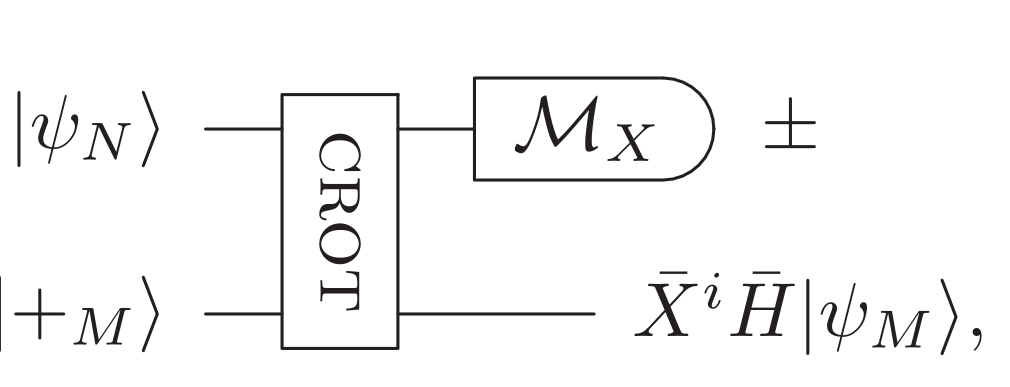
\includegraphics[scale=0.15]{teleportation_circuit.png}
    \label{fig:teleportaion_circuit}
    \caption{Teleportation circuit.}
\end{figure}
where $|\psi_N\rangle=\alpha\lgczero_N+\beta\lgcone_N$ and $|\psi_M\rangle=\alpha\lgczero_M+\beta\lgcone_M$. Upon the measurement in the $\lgcX$ basis, a logical Hadamard gate or $\bar{X}\bar{H}$ gate is applied to the data. Let us see why this is the case. For simplicity let us drop the bar notation for the encoded logical state.
\begin{align}\label{teleport_eqns}
    \CR_{NM}(|\psi_N\rangle \otimes |+_M\rangle) &= \dfrac{1}{\sqrt{2}}\CR_{NM}(\alpha|0_N0_M\rangle+\alpha|0_N1_M\rangle +\beta|1_N0_M\rangle +\beta|1_N1_M\rangle)\notag\\
    &=\dfrac{1}{2}\left[|+_N\rangle\left((\alpha+\beta)|0_M\rangle + (\alpha-\beta)|1_M\rangle\right)+|-_N\rangle\left((\alpha-\beta)|0_M\rangle+(\alpha+\beta)|1_M\rangle\right)\right] 
\end{align}
Note that $\bar{H}|\psi_M\rangle=1/\sqrt{2}\left[(\alpha+\beta)|0_M\rangle+(\alpha-\beta)|1_M\rangle\right]$ and $\bar{X}\bar{H}|\psi_M\rangle=1/\sqrt{2}\left[(\alpha-\beta)|0_M\rangle+(\alpha+\beta)|1_M\rangle\right]$, we can rewrite Eq. (\ref{teleport_eqns}) as 
\begin{align}
    \CR_{NM}(|\psi_N\rangle\otimes|+_M\rangle)=\dfrac{1}{\sqrt{2}}(|+_N\rangle(\bar{H}|\psi_M\rangle)+|-_N\rangle(\bar{X}\bar{H}|\psi_M\rangle))
\end{align}
Hence the teleportation circuit. Note that repetitions of $X$ and $H$ cannot generate the Clifford group. We need the $T$ gate. This can be done using the following circuit. 
\begin{figure}[h!]
    \centering
    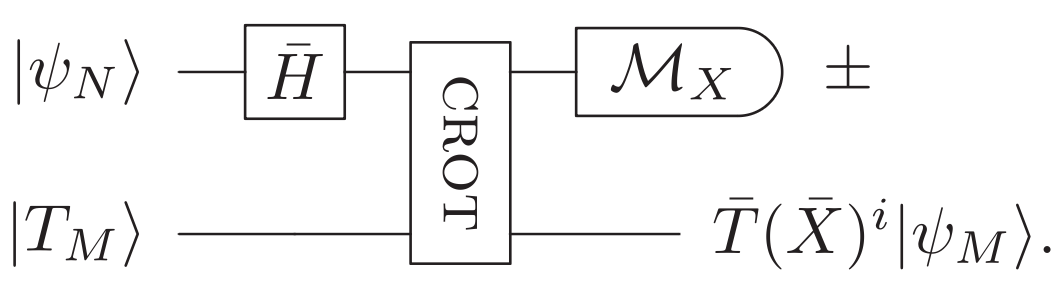
\includegraphics[scale=0.17]{teleportation_T.png}
    \label{fig:teleportaion_circuit_T}
    \caption{Teleportation circuit that generates the Clifford group.}
\end{figure}
This circuit requires an encoded $|T_M\rangle$ state. 
\section{Modular number measurement}
The $\CR$ gate is a fundamental building block for the universal gate set, state breeding, and the error correction scheme to be introduced. Here we'll look at a case where the $\CR$ gate can be used to perform a nondestructive modular measurement (MM) of excitation number $\hat{n}$. It's (MM) interesting because of two things. First, it's novel. Second, it can be used to both detect number-shift errors on an encoded state and to conditionally prepare $N$-fold rotation-symmetric codewords from a primitive state $|\Theta\rangle$. 

A nondestructive measurement of $\hat{n}$ mod $N$ can be performed with the following circuit,
\begin{figure}[h!]
    \centering
    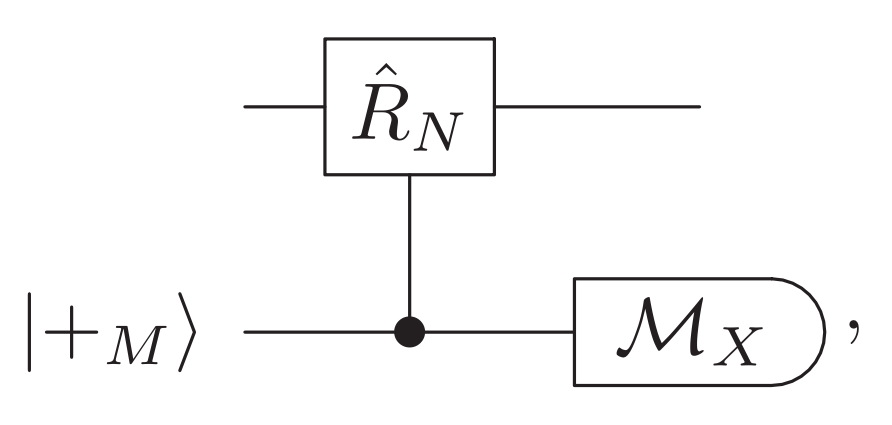
\includegraphics[scale=0.15]{images/modular_phase_number.png}
    \label{fig:modular_phase_number}
\end{figure}
where the controlled-$\hat{R}_N$ is defined as
\begin{align}
    \hat{C}_{R_N} = \CR_{NM/2} = e^{i(2\pi/NM)\hat{n}\otimes \hat{n}}
\end{align}
Let us see how this circuit works as intended. The top rail is the data rail (target), and $\lgcplus=|+_M\rangle$ is the ancillae (control),
\begin{align}
    \CR_{NM/2}(|n\rangle\otimes |+_M\rangle)&=e^{i(2\pi/NM)\hat{n}\otimes \hat{n}}(|n\rangle \otimes \sum_{k}c_k|m\rangle)\\
    &=e^{i(2\pi/NM)\hat{n}}|n\rangle \otimes e^{i(2\pi/NM)\hat{n}} |+_M\rangle\\
    &=|n\rangle \otimes e^{i(2\pi/NM)n}e^{i(2\pi/NM)\hat{n}} |+_M\rangle
\end{align}
Now, we make use of the fact that $n$ can be written as $n=\ell + pN$. This is simply for the sake of mathematical convenience. 
\begin{align}
    \CR_{NM/2}(|n\rangle\otimes |+_M\rangle) &=|n\rangle\otimes e^{i(\ell/N)(2\pi/M)\hat{n}}|+_M\rangle.
\end{align}
where $\ell$ is precisely $n$ mod $N$. We see that, the net result is a rotation of angle $\theta_{anc}=2\pi l/NM$ on the ancillae. This takes the ancillae out of the codespace, and hence allows for detection using a destructive phase measurement of the ancillae with resolution set by its embedded phase uncertainty $\Delta_M(\theta)$. When you know $\ell$, you \textit{know} $n$ mod N. 

For illustration, here we look at a $\hat{n}$ mode 4 measurement using two different ancillae: (a) a coherent state and (b) a two-lobe cat state. 
\begin{figure}[h!]
    \centering
    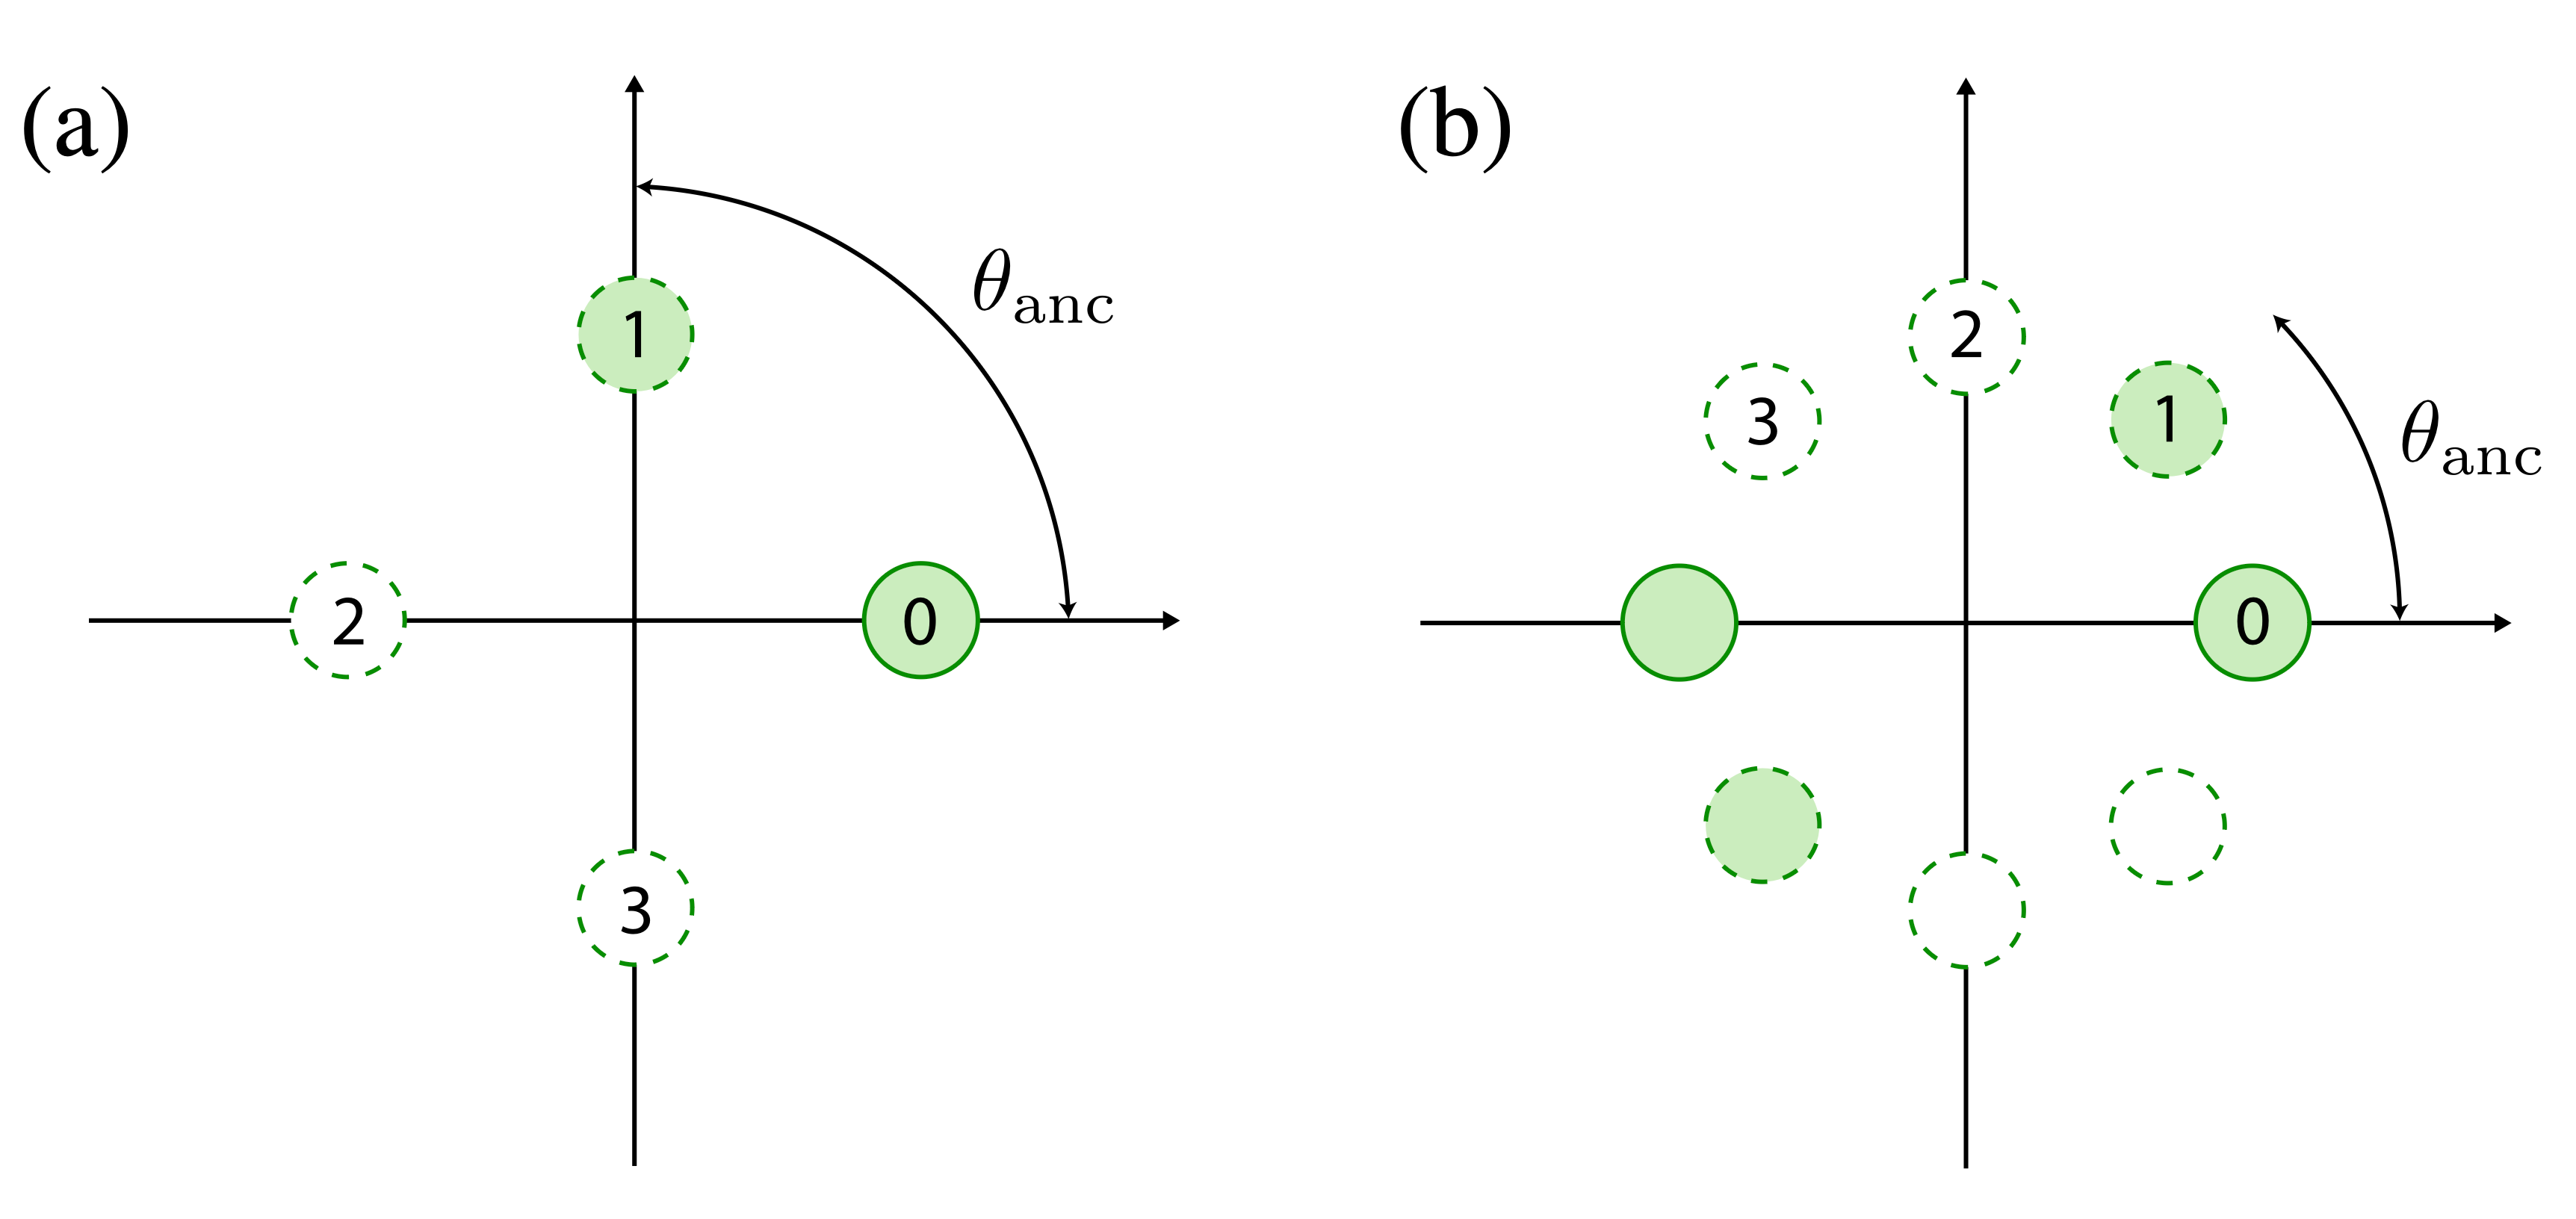
\includegraphics[scale=0.2]{images/modular_phase_measurement_example.png}
    \label{fig:modular_phase_number_example}
\end{figure}
Note that the $|+_M\rangle$ can only be rotated by $2\pi\ell/(NM)$.

For the coherent state, it's only a blob in the phase-space, hence a $1$-fold symmetric state.
\begin{itemize}
    \item Can we perform an $\hat{n}$ mod 1 measurement? All numbers mod 1 is zero. Thus, regardless of $n$, the coherent state would never rotate.
    \item Can we perform an $\hat{n}$ mod 2 measurement? If $n=0$, then $0$ mod $2=0$, which means the coherent state would not be rotating. If $n=1$, $1$ mod $2=1$. Now the state is going to rotate, by how much? Note that a coherent state is only a blob, and by design it is a $1$-fold symmetric state, i.e $M=1$. 
        \begin{align}
            \theta_{anc}=\dfrac{2\pi\ell}{NM}=\dfrac{2\pi}{2}=\pi
        \end{align}
        So, the coherent state is going to be rotated by $\pi$! What if $n=2$? $2$ mod $2=0$. Again, this means the coherent state is not going to be rotated. This logic carries for all $n$ above. Even $|n\rangle$ state can be measured, but can't be distinguished.
    \item Can we perform an $\hat{n}$ mod 3 measurement scheme? Yes, the values of $\ell$ are $0, 1, 2$, corresponds to
        \begin{align}
            \theta_0 = 0,\quad\theta_1=\dfrac{2\pi}{3},\quad\theta_2=\dfrac{4\pi}{3}.
        \end{align}
        [\textcolor{red}{I guess there's a bit of asymmetry here?}. \textcolor{blue}{No. I made a mistake.}]
    \item Can we perform an $\hat{n}$ mod 4 measurement scheme? Yes, the values of $\ell$ are $0, 1, 2, 3$, corresponds to
        \begin{align}
            \theta_0 = 0,\quad\theta_1=\dfrac{\pi}{2},\quad\theta_2=\pi,\quad\theta_3=\dfrac{3\pi}{2}.
        \end{align}
    \item For the sake of generalization, let us consider $\hat{n}$ mod 5. The values of $\ell$ are $0, 1, 2, 3, 4$.
        \begin{align}
            \theta_0 = 0,\quad\theta_1=\dfrac{2\pi}{5},\quad\theta_2=\dfrac{4\pi}{5},\quad\theta_3=\dfrac{6\pi}{5},\quad\theta_4=\dfrac{8\pi}{5}.
        \end{align}
\end{itemize}
Let us analyze the case for the two-lobe cat state. By design, the logical codewords are stabilized by $\hat{R}_2=e^{i\pi\hat{n}}$. Note that it is different from the previous case where $M=1$. The degree of symmetry here is larger.
\begin{itemize}
    \item We still cannot do $\hat{n}$ mod 1 measurement (it's a mathematical fact).
    \item We can perform an $\hat{n}$ mod 2 measurement. It corresponds to 
        \begin{align}
            \theta_0=0,\quad\theta_1=\dfrac{\pi}{2}.
        \end{align}
        If you make a phase measurement of $e^{i\theta\hat{n}}|+_M\rangle$ and $\theta=\pi/2$, then the number of excitation are $2k+1$, where $k$ is an integer.
    \item We can do $\hat{n}$ mod 3 measurement. It corresponds to
        \begin{align}
            \theta_0=0,\quad\theta_1=\dfrac{\pi}{3},\quad\theta_2=\dfrac{2\pi}{3}
        \end{align}
        If you make a phase measurement of $e^{i\theta\hat{n}}|+_M\rangle$ and $\theta$ turns out to be 0, then the number of excitation are $0, 3, 6, 9,\dots=3k+0$ for $k$ integers. If $\theta$ turns out to be $\pi/3$, $\ell=1$, and thus the number of excitation are $3k+1$, for $k$ integers. If $\theta$ turns out to be $2\pi/3$, $\ell=2$, and thus the number of excitation are $3k+2$, for $k$ integers.  
\end{itemize}
\subsection*{Error propagation in modular number measurement}
Rotation errors on the ancillae $|+_M\rangle$ during the $\hat{n}$ mod $N$ measurement do not propagate to the data rail. However, any ancillae error that does \textit{not} commute with $\hat{n}$, such as loss or gain, can introduce \textit{rotation errors} on the data rail (we postpone the why's and the how's for now). For example, a loss error at a random time during the measurement leads to a rotation error of the data rail by an angle $\theta_{data}\in [0, 2\pi/NM)$. Worst case scenario, the data qubit suffers a rotation $\to e^{i(2\pi/NM)\hat{n}}$. The rotation angle is small when $M$ large, but conversely is large when $M$ is small. At $M=1$ (such as a coherent state), the rotating angle is $\to 2\pi/N$, which is equivalent to a completely randomized phase rotation. A small error on the ancillae qubit is thus propagated and amplified on the data qubit.

On the other hand, using a large $M$ ancillae brings about disadvantages too: large measurement uncertainty. Note that this is \textit{not} the embedded phase uncertainty, but the fact that as you increase the degree of symmetry of the ancillae, the rotation angle $\theta_{anc}=2\pi\ell/NM$ is reduced, making it harder to distinguish the differences between different $\ell$. [\textcolor{red}{What can I learn from this?}]
\section{Errors and error propagation}
The discussion of fault tolerance (FT) of bosonic codes differ from that of sabilizer codes. In bosonic codes, bosonic modes are allowed to have small errors. How small they should be? Below the code's number $N$ and rotational distance $\pi/N$. For this reason, propagation of \textit{small errors} is not a major issue. What's dangerous is instead, amplification of small errors.

As we shall see, the gates introduced in the previous section don't amplify errors. They don't amplify the magnitude of a number-shift error of the form $\sim\hat{a}^k$ (although they might map a number-shift error onto a number-shift error plus a rotation error $e^{i\theta\hat{n}}$). The new rotation error is proportional to the size of the number-shift error relative to the Fock-space distance $\theta\sim k/N$. 
\subsection{Error bases and large vs small errors}
There are two single-mode operator bases that are useful in the context of rotation codes. The first is the set,
\begin{align}
    \{\hat{n}^{\ell}\hat{a}^{k}, (\hat{a}^\dagger)^k\hat{n}^\ell\}
\end{align}
Note that $(\hat{n}^{\ell}\hat{a}^{k})^\dagger = (\hat{a}^\dagger)^k\hat{n}^\ell$. The reason: the displacement operator can be expanded in normal ordered form, and the normal ordered form can be written in terms of the set, and in turn any Kraus operators of any single-mode channel can be written in the operator basis formed by the displacement operators. 

A second useful operator basis is 
\begin{align}
    \{e^{i\theta\hat{n}}\hat{a}^k, (\hat{a}^\dagger)^k e^{-i\theta\hat{n}}\},
\end{align}
where $k\leq 0$ is an integer and $\theta\in [0, 2\pi)$. Since we're going to use it many times, here's a shorthand notation,
\begin{align}
    \hat{E}_k(\theta)=\begin{cases}
        e^{i\theta\hat{n}}\hat{a}^{|k|},& k < 0,\\
        (\hat{a}^\dagger)^{|k|}e^{-i\theta\hat{n}}, &k\leq 0.
    \end{cases}
\end{align}
A non-negative $k$ thus denotes an upward shift in number, while a negative $k$ means a downward shift in number.

Now we discuss what's considered as a large error and what's considered as a small error. First, an error of the form $\hat{E}_k(\theta)$ is detectable for any rotation code of order $N$, provided that $0<|k|<N$. Second, because of the embedded phase uncertainty, we wouldn't be able to make a statement about the detectability of phase errors. For ideal NP codes (i.e. $\Delta_N(\theta)\to 0$, a pure rotation error $\hat{E}_0(\theta)$ should be detectable, provided that $0<\theta<\pi/N$. Intuitively, a number-shift error with value of $|k|$ small compared to $d_N/2$ should be called small, and phase-shift error $|\theta|$ small compared to $d_\theta/2$ should be called small.
\subsection{Error propagation}
This subsection explains how errors propagate through gates introduced previously. The gates $\{\hat{S}_N,\CR_{NM}\}$ will be shown that, although they are generated by quadratic powers of the number operator $\hat{n}$ and non-Gaussian, they do not amplify errors too badly.

All gates in our scheme commute with pure rotation errors $\hat{E}_0(\theta)$ [\textcolor{red}{Q: Why then? Is it obvious?} \textcolor{blue}{A: The necessary set consists of $\hat{S}, \hat{C}_Z\equiv \CR$. Because they are all generated by quadratic powers of the number operator, it's quite obvious that they commute with $e^{i\theta \hat{n}}$, since $[e^{A}, e^B]=0$ if $[A,B]=[\hat{n}^k, \hat{n}^l]$ for all $k, l$}]. For number-shift errors, we use the following identity,
\begin{align}\label{commutation_relation}
    e^{c\hat{n}^\ell}\hat{a}^k = e^{c[n^\ell-(n+k)^\ell]}\hat{a}^{k}e^{c\hat{n}^\ell}.
\end{align}
For upward-shift number errors, simply take the Hermitian conjugate of Eq. (\ref{commutation_relation}). A summary of how our gates interact with errors is presented in Fig. (\ref{fig:error_propagation}).\newline
\begin{figure}[h!]
    \centering
    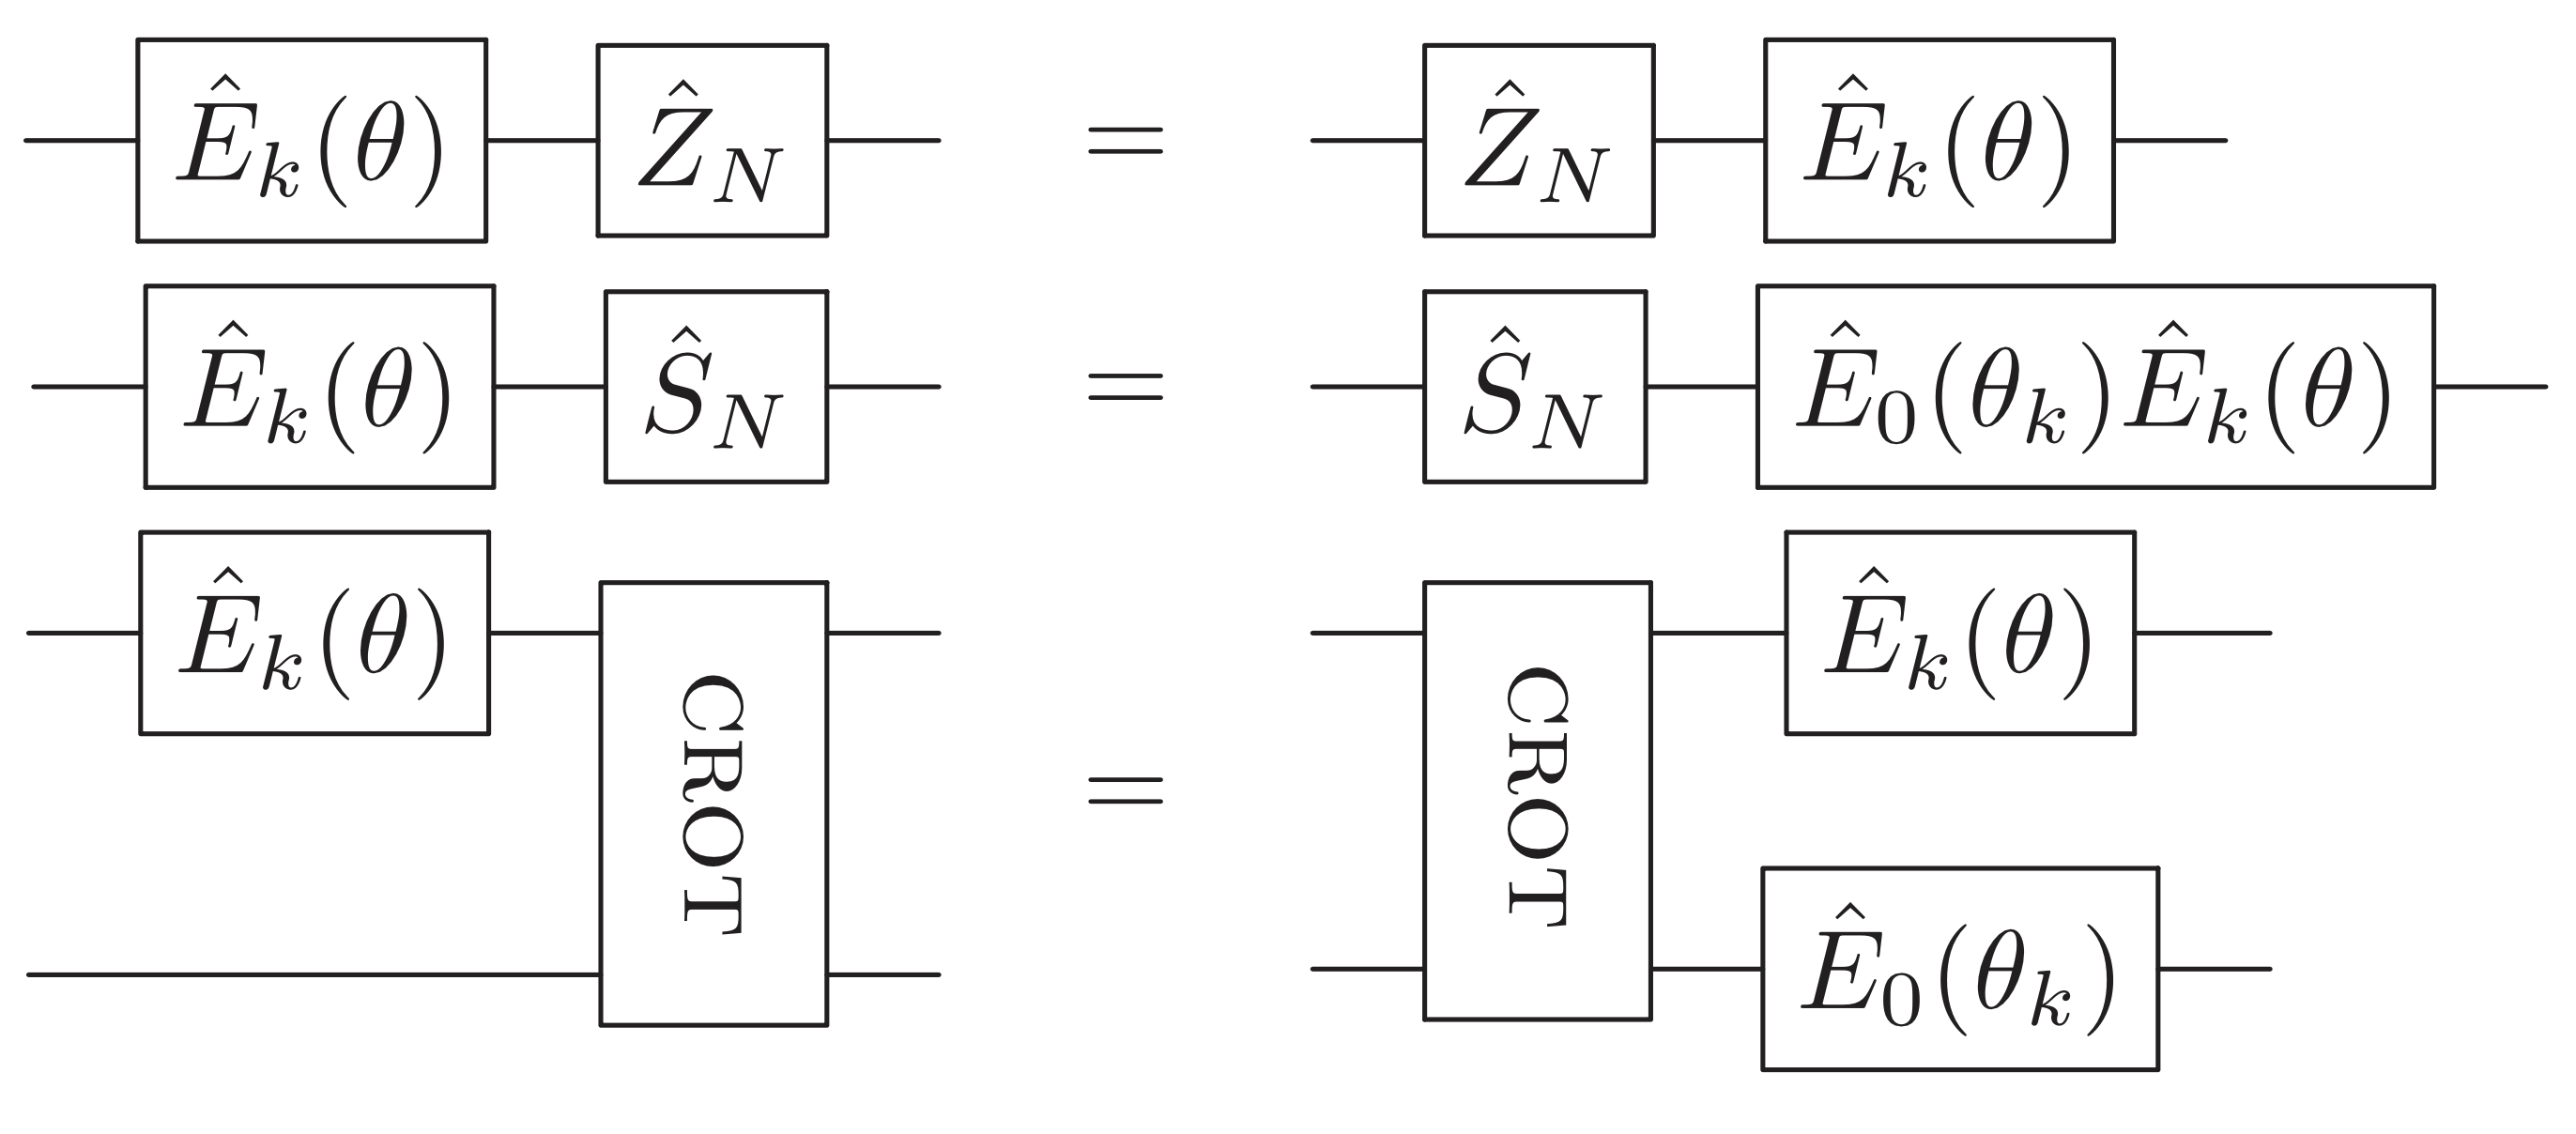
\includegraphics[scale=0.2]{images/error_propagation.png}
    \label{fig:error_propagation}
    \caption{How errors propagate.}
\end{figure}
For gates with $\ell=1$, i.e. $e^{c\hat{n}}$ (where $c$ is a complex number), such as a $\hat{Z}$ rotation, the prefactor of Eq. (\ref{commutation_relation}) is simply a global phase. Hence propagating an error $\hat{E}_k(\theta)$ through a Gaussian $\hat{Z}$ does not amplify it [\textcolor{olive}{C: It's probably a good time to stop an reflecting what does it mean by \textit{propagation}. It is as if the error is being \textit{swapped} with the gate along the chronological direction. This `action' of swapping is essentially described by the commutation!?}]. 

For gates with $\ell=2$, i.e. $e^{c\hat{n}^2}$ (non-Gaussian) such as the gate $\hat{S}_N$, the prefactor becomes,
\begin{align}
    \hat{S}_N \hat{E}_k(\theta) = \begin{cases}
        e^{-i(k^2\pi/N^2)}\hat{E}_k\left(\theta+\dfrac{\pi k}{N^2}\right)\hat{S}_N,\quad k < 0,\\[10pt]
        e^{+i(k^2\pi/N^2)}\hat{E}_k\left(\theta+\dfrac{\pi k}{N^2}\right)\hat{S}_N,\quad k \geq 0
    \end{cases}
\end{align}
Here, the global phases introduced by error propagation are different for upward/downward-shift errors. However, the important thing is the error is being amplified by $\pi k/N^2\propto k$. This is a linear increase, and thus for small, approximately correctable errors the amplification should not be a problem.  

Now we come to the interesting case, the $\CR$ gate. Propagating une error $\hat{E}_k(\theta)$ through $\CR$ gate introduces new errors onto the other mode. More specifically, suppose that we have the $a$ mode encoded in an order-$N$ rotation code and the $b$ mode encoded in an order-$M$ rotation code, then
\begin{align}
    \CR_{NM} \hat{E}^a_k(\theta) = \hat{E}^a_k(\theta)\hat{E}^b_0\left(\dfrac{\pi k}{NM}\right)\CR_{NM}.
\end{align}
Here, the initial number-shift error on mode $a$ spreads to a rotation error on mode $b$ [\textcolor{red}{Q: Can you prove this?} \textcolor{blue}{A: Here's what I have in mind}]. Here's why
\begin{align}
    \CR_{NM} \hat{E}^a_k(\theta)&= e^{i(\pi/NM)\hat{n}_a\otimes\hat{n}_b}e^{i\theta\hat{n}_a}\hat{a}^{|k|}\\
    &=e^{i\theta\hat{n}_a}e^{i(\pi/NM)\hat{n}_a\otimes \hat{n}_b}a^{|k|}\quad\text{\textcolor{olive}{(True because $a$ and $b$ are two distinct modes)}}\\
    &=e^{i\theta\hat{n}_a}e^{i(\pi/NM)\hat{n}_a\otimes \hat{n}_b}a^{|k|}e^{-i(\pi/NM)\hat{n}_a\otimes \hat{n}_b}e^{i(\pi/NM)\hat{n}_a\otimes \hat{n}_b}
\end{align}
Now what we need to prove is essentially $e^{i(\pi/NM)\hat{n}_a\otimes\hat{n}_b}\hat{a}^{|k|}e^{-i(\pi/NM)\hat{n}_a\otimes\hat{n}_b}$. This can be proven using the BCH lemma, since we're essentially doing a unitary transformation here. The formula states that 
\begin{align}
    e^{cX}Y e^{-cX}=\sum_{m=0}^{\infty} \dfrac{[(cX)^m, Y]}{m!},
\end{align}
where the iterated commutator is defined as $[(cX)^m, Y]\equiv [cX, \dots [cX,[cX, Y]]\dots]$. Here,
\begin{align}
    [c\hat{n}_a\otimes\hat{n}_b, \hat{a}_a\otimes \hat{\mathbb{1}}_b] &= [c\hat{n}_a, \hat{a}_a]\otimes\hat{n}_b\\
    &=(c\hat{a}_a^\dagger\hat{a}_a\hat{a}_a-\hat{a}_a\hat{a}_a^\dagger\hat{a}_a c)\otimes \hat{n}_b\\
    &=-(c\hat{a}_a\hat{a}_a^\dagger\hat{a}_a-c\hat{a}_a^\dagger\hat{a}_a\hat{a}_a)\otimes \hat{n}_b\\
    &=-[c\hat{a}_a, \hat{a}_a^\dagger]\hat{a}_a\otimes \hat{n}_b\\
    &=-c\hat{a}_a\otimes \hat{n}_b
\end{align}
One more time,
\begin{align}
    [c\hat{n}_a\otimes \hat{n}_b, -c\hat{a}_a\otimes \hat{n}_b]&=-[c\hat{n}_a\otimes \hat{n}_b,c\hat{a}_a\otimes \hat{n}_b]\\
    &=c^2\hat{a}_a\otimes \hat{n}_b^2
\end{align}
By induction, 
\begin{align}
    e^{c\hat{n}_a\otimes\hat{n}_b}(\hat{a}_a\otimes \hat{\mathbb{1}}_b)e^{-c\hat{n}_a\otimes\hat{n}_b}&=\sum_{m=0}^\infty \dfrac{c^m \hat{a}_a\otimes \hat{n}_b^m}{m!}\\
    &=\hat{a}_a\otimes e^{c\hat{n}_b}
\end{align}
Now, $(UAU^{-1})^{k}=UAU^{-1}UAU^{-1}\cdots AU^{-1}=UA^{k}U^{-1}$, while $(\hat{a}_a\otimes e^{c\hat{n}_b})^k=\hat{a}^{k}_a\otimes e^{kc\hat{n}_b}$. That means
\begin{align}
\CR_{NM}\hat{E}_k^a(\theta)&=e^{i\theta\hat{n}_a}e^{i(\pi/NM)\hat{n}_a\otimes \hat{n}_b}a^{|k|}e^{-i(\pi/NM)\hat{n}_a\otimes \hat{n}_b}e^{i(\pi/NM)\hat{n}_a\otimes \hat{n}_b}\\
&=e^{i\theta\hat{n}_a}\hat{a}_a^{|k|}e^{i(k\pi/NM)\hat{n}_b}e^{i(\pi/NM)\hat{n}_a\otimes\hat{n}_b}\\
&=\hat{E}_k^a(\theta)\hat{E}_0^b\left(\dfrac{\pi k}{NM}\right)\CR_{NM}
\end{align}
\section{The question needed an answer}
OK. We've seen that an error $\hat{E}_k^a(\theta)$ on mode $a$ can propagate through the $\CR$ gate and then enacts a measurable phase error $\exp(\pi k/NM)$ on mode $b$. From one perspective, this is unfortunate because the error has been propagated further to other modes. From another perspective, this can be utilized to detect loss errors on mode $A$.

Let us now call mode $a$ as data mode $d$ and $b$ as the ancillary mode $\text{anc}$. Our goal is to detect loss error $\hat{E}_k^d(\theta)$ using phase measurement on the ancillary mode. Here's the million-dollar question: \textcolor{red}{What's the input state on the ancillary rail that maximizes the fidelity of the loss detection measurement?}
\subsection{Criteria}
Here's a list of criteria that we're looking for in a candidate,
\begin{itemize}
    \item Regardless of the degree of symmetry, we'll still always have to look at the phase uncertainty $\Delta(\theta)$, which is a generic properties of all the states that we're looking at. Because we'll need to make a measurement on the ancillae input to detect loss from the data input, and the measurement itself is in the $\bar{X}$ basis, it follows that the state should have a inherently small phase uncertainty to begin with. \textcolor{olive}{If the state is characterized as a state with $N$-fold symmetry--i.e. a RSBC code, then the phase uncertainty is calculated using the Fock-grid coefficients of the code. If the state itself is not a RSBC code, then we resort to the original calculation, which is cumbersome, but not impossible.} 
    \item At this stage, we care only about the canonical phase measurement, i.e. described by the complete set of POVMs constructed from the phase state 
    \begin{align}|\phi\rangle=\dfrac{1}{\sqrt{2\pi}}\sum_{n=0}^\infty e^{in\phi}|n\rangle\end{align}
\end{itemize}
\subsection{Candidate 1: Encoded logical plus state of an order-$M$ RSBC code}
We'll first look at the encoded logical plus state of an order-$M$ code, $\lgcplus_M\equiv |+_M\rangle$. By definition, it has support on every $M$-th Fock states,
\begin{align}
    \psianc\equiv |+_{M,\textsc{code}}\rangle &= \sum_{\ell=0}^\infty c_{\ell M}|\ell M\rangle\\
    &=\dfrac{1}{\sqrt{N_+}}\sum_{m=0}^{M-1}e^{i(2m\pi/M)\hat{n}}|\Phi'\rangle,
\end{align}
where $N_+$ is normalization constants and the primitive state is $|\Phi'\rangle$. Note that this primitive state is the weighted superposition of the original primitive $|\Phi\rangle$ with itself being rotated by $\pi/M$ (See Appendix). Having determined the state of the ancillary component, suppose we have a downward number-shift of $k$ on the input mode, which we assume to be an order-$N$ code, this introduces a rotation on the ancillae
\begin{align}
    \exp\left(\dfrac{\pi k}{NM}\hat{n}\right)\psianc &= \dfrac{1}{\sqrt{N_+}}\sum_{m=0}^{M-1}\exp\left(i{\dfrac{\pi k}{NM}\hat{n}}\right)\exp\left({i\dfrac{2m\pi}{M}\hat{n}}\right)|\Phi'\rangle\\
    &=\dfrac{1}{\sqrt{N_+}}\sum_{m=0}^{M-1}\exp\left[i\left(\dfrac{k}{N}+2m\right)\dfrac{\pi}{M}\hat{n}\right]|\Phi'\rangle
\end{align}
Essentially we're having the following questions,
\begin{itemize}
    \item[\textcolor{red}{Q1.}] By design, for an order-$N$ rotation symmetric code, i.e. the code distance is $d_N=N$, a loss error much be smaller than its distance $k<d_N$ to be detectable (by means of number measurement, $\langle \hat{n}\rangle$ must be a multiple integer of $N$). Can we increase this bound? \textcolor{olive}{(Actually I'm quite confused by the fact that $k<d_N$. Is there a hidden `preferred' word lurking somewhere?. Is it related to the correctability of the code? Because isn't $k$ just don't have to be multiple integer of $N$?)}
    \item[\textcolor{red}{Q2.}] Which scheme is more advantageous? (a) $M>N$; (b) $M=N$; or (c) $M<N$. 
\end{itemize}
\begin{itemize}
    \item[\textcolor{blue}{A1.}] Because we're using the encoded plus state $\psianc=|+_K\rangle$, which is a $+1$ eigenstate of the rotation operator $\widehat{\exp}[i(2\pi l)\hat{n}/M]$, and a phase measurement only care about $\theta$ mod $2\pi/M$, it follows that we can detect a shift $k$ if and only if $k$ mod $2N\neq 0$. There's also a gap between the maximum number of $k$ that's detectable. More specifically, $N \leq k<2N$, i.e. $N$ more number-shift errors can be detected using the proposed measurement scheme.     
    \item[\textcolor{blue}{A2.}] Because the magnitude of rotation scales as $1/M$, it is advantageous to stick to small $M$, which results in larger gaps in rotation distances between different $k$. This is equivalent to using $M<N$ and $N\geq 2$, where $M=2$ is the most optimal value (from this perspective) for all RSB codes.  
\end{itemize}

\section{Two-mode bosonic gate}
We first consider a system of one linear cavity mode with frequency $\omega_a$ coupled to a transmon ancilla. The system Hamiltonian reads
\begin{align}
    H = H_{\text{cav}} + H_{\text{anc}} + H_{\text{drive}} + H_{\text{int}},\\
    H_{\text{cav}} = \omega_a \hat{a}^\dagger \hat{a},\\
    H_{\text{anc}} = 4E_C\hat{n}^2 - E_J\cos\hat{\phi},\\
    H_{\text{drive}} = -2e\hat{n}V_d \sin(\omega_d t + \theta_{d}),\\
    H_{\text{int}} = -2e\hat{n}V_a(a^\dagger + a)  
\end{align}
We'll deal with the cosine expansion now. Can we just simply keep everything? If we do, let's consider how to do it. Let us denote 
\begin{align}
    \hat{\phi} = \left(\dfrac{2E_C}{E_J}\right)^{1/4}(c^\dagger +c),
    \hat{n} = \dfrac{i}{2}\left(\dfrac{E_J}{2E_C}\right)(b^\dagger - b).
\end{align}

\begin{align}\label{eqn:singlegate}\displaystyle
    \hat{H}= (\omega_q-\omega_d)\hat{\sigma}_z+\dfrac{\Omega_R}{2}\left(\cos\phi\hat{\sigma}_x+\sin\phi\hat{\sigma}_y\right).
\end{align}

\bibliographystyle{plain} % We choose the "plain" reference style
\bibliography{refs}
\end{document}
